Nós vemos, nas figuras 1 e 2, exemplos de bloqueio de tela de um telefone celular que só funciona com uma senha que não é digitada, mas desenhada com segmentos de reta. Esses segmentos formam uma linha poligonal com vértices em um reticulado. Ao desenhar o padrão correspondente à senha, o dedo deve permanecer todo o tempo tocando a tela. Toda a linha poligonal corresponde a uma sequência de algarismos e essa sequência é que é, de fato, a senha. O traçado das poligonais obedece às regras a seguir:

\begin{itemize}

\item[a)] O traçado começa por um dos pontos destacados, os quais correspondem aos algarismos de 1 a 9 (figura 3).

\item[b)] Cada segmento do padrão deve ter como um dos seus extremos (aquele em que terminamos de traçar o segmento) um ponto que ainda
não foi usado.

\item[c)] Se um segmento liga dois pontos e contém um terceiro (o seu ponto médio), então o algarismo correspondente a esse terceiro ponto é incluído na senha. Isso não acontece quando esse ponto/algarismo já foi usado.

\item[d)] Toda senha tem pelo menos quatro algarismos.

\end{itemize}

\begin{center}
    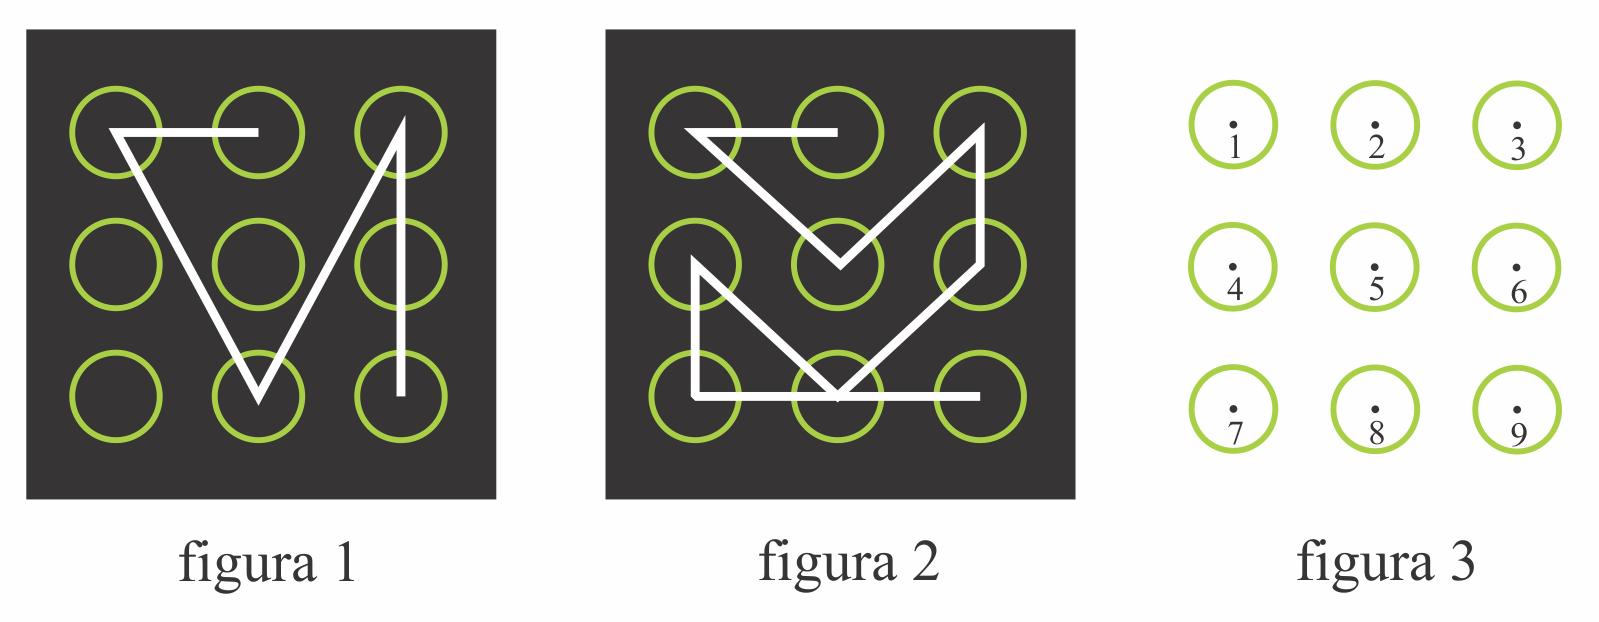
\includegraphics[width = 0.5\textwidth]{figura.png}
\end{center}


Assim, toda linha poligonal é associada a uma sequência de quatro ou mais algarismos, os quais aparecem na senha na mesma ordem em que são visitados. Na figura 1 acima, por exemplo, a senha é 218369, caso o
primeiro ponto visitado tenha sido o 2. Note que o segmento ligando os pontos associados aos algarismos 3 e 9 inclui o ponto associado ao algarismo 6. Se o primeiro ponto visitado fosse o 9, então a senha seria 963812. Se o primeiro ponto visitado fosse o 6, então a senha seria 693812. Note que o 6 seria pulado, já que não poderia repetir. Por outro lado, a linha poligonal da figura 2 é associada a uma única senha.

Determine o menor $n \ge 4 $ tal que dado qualquer subconjunto de n algarismos de 1 a 9 é possível elaborar uma senha que envolva exatamente esses algarismos em alguma ordem.